\documentclass[10pt,a4paper]{article}

\usepackage[T1]{fontenc}
\usepackage{lmodern}
\usepackage[margin=2cm]{geometry}
\usepackage{microtype}
\usepackage{amsmath}
\usepackage{booktabs,tabularx,longtable,array}
\usepackage[table]{xcolor}
\usepackage{enumitem}
\usepackage{float}
\usepackage[font=small,skip=4pt]{caption}
\usepackage{parskip}
\usepackage{titlesec}
\usepackage{pdflscape}
\usepackage{tikz}
\usetikzlibrary{positioning,arrows.meta,shapes.geometric,shapes.misc,fit,backgrounds,calc}
\usepackage[colorlinks=true,linkcolor=blue!50!black,urlcolor=blue!50!black]{hyperref}

\makeatletter
\g@addto@macro{\UrlBreaks}{\do\/\do-\do\_\do\?\do\=\do\&\do\.\do\a\do\b\do\c\do\d\do\e\do\f\do\g\do\h\do\i\do\j\do\k\do\l\do\m\do\n\do\o\do\p\do\q\do\r\do\s\do\t\do\u\do\v\do\w\do\x\do\y\do\z}
\makeatother

\definecolor{kfcblue}{HTML}{185FA5}
\definecolor{kfcteal}{HTML}{0F6E56}
\definecolor{kfcpurple}{HTML}{534AB7}
\definecolor{kfcgray}{HTML}{5F5E5A}
\definecolor{lightblue}{HTML}{E6F1FB}
\definecolor{lightteal}{HTML}{E1F5EE}
\definecolor{lightpurple}{HTML}{EEEDFE}
\definecolor{lightgray}{HTML}{F1EFE8}
\definecolor{lightamber}{HTML}{FAEEDA}

\titleformat{\section}{\large\bfseries\color{kfcblue}}{\thesection}{0.6em}{}
\titleformat{\subsection}{\normalsize\bfseries}{\thesubsection}{0.6em}{}
\titlespacing*{\section}{0pt}{10pt}{4pt}
\titlespacing*{\subsection}{0pt}{6pt}{2pt}
\setlist{itemsep=1pt,topsep=2pt,parsep=0pt}
\renewcommand{\arraystretch}{1.15}
\newcolumntype{L}[1]{>{\raggedright\arraybackslash}p{#1}}
\newcolumntype{Y}{>{\raggedright\arraybackslash}X}
\pagestyle{plain}

\newcommand{\ep}[1]{\texttt{\small #1}}
\newcommand{\eu}[1]{{\small\nolinkurl{#1}}}

\begin{document}

\begin{titlepage}
\centering
\vspace*{\fill}
{\Huge\bfseries\color{kfcblue} GameTrend Radar\par}
\vspace{0.4cm}
{\Large Real-time trend analytics for Roblox and Steam games\par}
\vspace{2.5cm}
{\Large\bfseries Team KFC\par}
\vspace{0.5cm}
{\large
Bart\l{}omiej Borycki\\[3pt]
Micha\l{} Iwaniuk\\[3pt]
Jan Cwalina\\[3pt]
Mi\l{}osz Choda\'n\par}
\vspace*{\fill}
\end{titlepage}

%======================================================================
\section{Project deliverables (user's perspective)}
Roblox is a trend-driven game platform with a very young audience (mostly 10--15 years old). New mechanics spread within days, and many of them are copied from Steam hits. \textbf{Users} are independent Roblox developers, small studios and game-market analysts who want to know what is rising now, where a trend came from, and how crowded a niche is.

\begin{itemize}
  \item \textbf{Dashboard} (web app) with four views:
  \begin{itemize}
    \item \emph{Trending now}: Roblox/Steam games ranked by trend score, with players, growth and a +3\,h projection; filters by genre and country.
    \item \emph{Steam$\rightarrow$Roblox opportunities}: trending Steam games released in the last 90 days, their automatically matched Roblox clones (with match confidence) and a saturation indicator.
    \item \emph{Game details}: metrics, player time series, linked Steam original and the timeline of its Roblox clones.
    \item \emph{Model and data health}: model accuracy compared with simple baselines, data freshness and API errors.
  \end{itemize}
  \item \textbf{Data platform} in a lambda architecture, run locally with \texttt{docker compose up}.
  \item \textbf{ML models:} a model that estimates how many players a game should have (the difference from the actual count is the trend score) and a trend model for short-term projection.
\end{itemize}
Only aggregated, public, game-level data is collected. There is no data about individual players.

%======================================================================
\section{Business process -- core use case}
Core use case: \textbf{``Find and assess a game trend opportunity''} (Figure~\ref{fig:bpmn} on page~\pageref{fig:bpmn}, BPMN~2.0). The developer browses ranked games, drills into one, and checks its Steam origin (release date, Roblox clones, saturation) or similar Roblox games. Steam$\rightarrow$Roblox matching is fully automatic. The data platform runs independently on a timer.



%======================================================================
\section{Data sources -- preliminary investigation}
All endpoints were probed with scripts on 17 Oct 2026. The figures below are \textbf{measured}. Both sources are free and need no API key.

\subsection{Roblox (primary stream)}
Public web APIs. The Games API is documented as a legacy API (\url{https://create.roblox.com/docs/cloud/legacy}). Discovery and search are undocumented website endpoints (random UUID as \ep{sessionId}).

{\small
\begin{longtable}{L{4.4cm} L{5.9cm} L{5.4cm}}
\toprule
\textbf{Endpoint} & \textbf{Attributes used} & \textbf{Purpose}\\
\midrule\endhead
\eu{apis.roblox.com/explore-api/v1/get-sorts?country=XX} & \ep{universeId, name, playerCount, totalUpVotes, totalDownVotes, isSponsored, genreL1}; 28 ranking lists per country & discovery of game IDs, per-country rank, cheap player counts\\
\eu{apis.roblox.com/search-api/omni-search?searchQuery=..} & \ep{universeId, name, description, playerCount, creatorId} (40 per query) & finding Roblox counterparts of Steam games\\
\eu{games.roblox.com/v1/games?universeIds=..} (50 IDs) & \ep{playing, visits, favoritedCount, maxPlayers, created, updated, genre\_l1, genre\_l2, creator} & core snapshot: concurrent players, cumulative visits, update events\\
\eu{games.roblox.com/v1/games/votes?universeIds=..} & \ep{upVotes, downVotes} & like ratio (model feature)\\
\bottomrule
\end{longtable}}

\subsection{Steam (second stream)}
\begin{sloppypar}Docs: \url{https://partner.steamgames.com/doc/webapi/ISteamUserStats}, \url{https://partner.steamgames.com/doc/webapi/ISteamChartsService}, \url{https://wiki.teamfortress.com/wiki/User:RJackson/StorefrontAPI}.\end{sloppypar}

{\small
\begin{longtable}{L{4.4cm} L{5.9cm} L{5.4cm}}
\toprule
\textbf{Endpoint} & \textbf{Attributes used} & \textbf{Purpose}\\
\midrule\endhead
\eu{ISteamUserStats/GetNumberOfCurrentPlayers/v1?appid=..} & \ep{player\_count} (1 game per call) & Steam player stream\\
\eu{ISteamChartsService/GetMostPlayedGames/v1} & \ep{rank, appid, last\_week\_rank, peak\_in\_game} (top 100, daily) & candidate games\\
\eu{store.steampowered.com/search/results/?filter=popularnew} & appid, title, release date (HTML in JSON, 100 per page) & recent releases, i.e.\ candidates for clone matching\\
\eu{store.steampowered.com/api/appdetails?appids=..} & \ep{name, release\_date, genres} & game metadata\\
\bottomrule
\end{longtable}}

\subsection{Data characteristics: type, volume, velocity}
\begin{table}[H]
\centering\small
\begin{tabularx}{\textwidth}{L{3.1cm} Y L{2.9cm} L{2.0cm}}
\toprule
\textbf{Feed} & \textbf{Measured} & \textbf{Planned read} & \textbf{Rows/day}\\
\midrule
Roblox ranking lists & 60 requests $\rightarrow$ 1,583 unique games (12 countries), $\sim$100\,kB/response, no throttling & every 15 min & $\sim$345k\\
Roblox game snapshots & $\sim$1.4\,kB/record; within 60\,s, \ep{playing} changed for 82\% and \ep{visits} for 94\% of games; HTTP 429 after $\sim$11 rapid requests & every 5 min, $\le$2,000 games & 576k\\
Roblox votes & 2,060 games in 30\,s without throttling; 25\% change per minute & every 15 min & 192k\\
Roblox search & 40 results/query & daily (clone candidates) & $<$4k\\
Steam current players & median 0.36\,s/call, about 100k calls/day allowed & every 15 min, $\le$500 games & 48k\\
Steam charts, store & top 100; 379 popular new releases; appdetails about 200 req/5 min & daily / new game & small\\
\bottomrule
\end{tabularx}
\caption{Base characteristics. All data is semi-structured JSON over HTTPS (REST polling). Average velocity is about 400--800 records/min.}
\end{table}

\textbf{Volume reduction.} Raw JSON would be about 1.4\,GB/day. We keep it much smaller:
\begin{itemize}
  \item producers keep only numeric fields (fact row \ep{ts, id, playing, visits, favorites, up, down}, about 50\,B),
  \item metadata is stored once and updated only on change,
  \item Kafka keeps raw messages for 24\,h,
  \item the master dataset is stored as Snappy-compressed Parquet,
  \item the serving DB keeps 5-min data for 14 days and hourly aggregates after that.
\end{itemize}
The result is about 1.2M rows/day ($\approx$10--15\,MB/day in Parquet), under 2\,GB per semester.

\begin{landscape}
\begin{figure}[p]
\centering
\resizebox{\linewidth}{!}{%
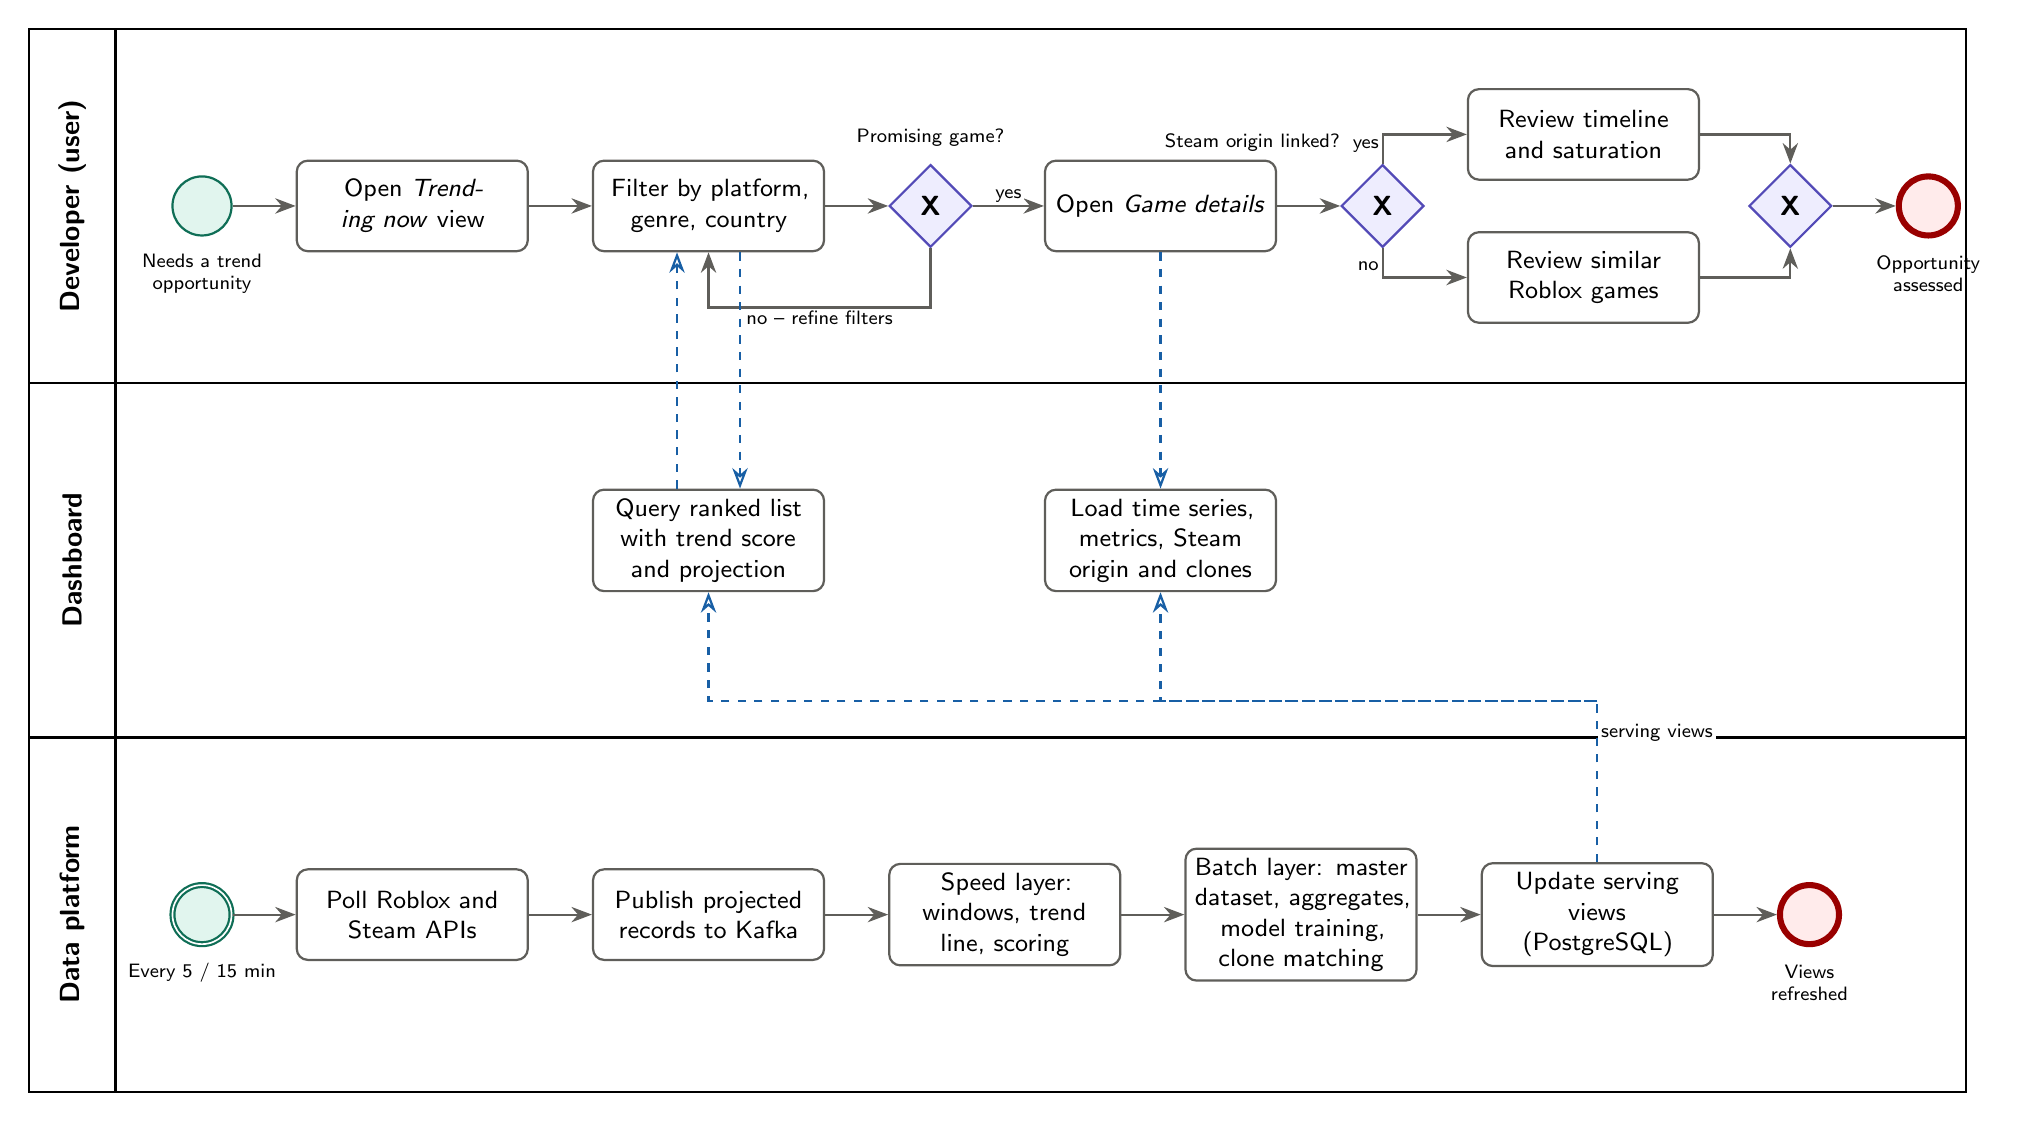
\begin{tikzpicture}[
  font=\sffamily\small,
  task/.style={rectangle, rounded corners=4pt, draw=kfcgray, fill=white, thick, minimum width=2.9cm, minimum height=1.15cm, align=center, text width=2.7cm},
  start/.style={circle, draw=kfcteal, thick, minimum size=0.75cm, fill=lightteal},
  timer/.style={circle, draw=kfcteal, double, thick, minimum size=0.75cm, fill=lightteal},
  endev/.style={circle, draw=red!60!black, line width=2.2pt, minimum size=0.75cm, fill=red!8},
  gw/.style={diamond, draw=kfcpurple, thick, fill=lightpurple, minimum size=1.05cm, inner sep=0pt, font=\sffamily\bfseries},
  flow/.style={-{Stealth[length=2.6mm]}, thick, draw=kfcgray},
  msg/.style={-{Stealth[length=2.6mm,open]}, dashed, thick, draw=kfcblue},
  lbl/.style={font=\sffamily\scriptsize, fill=white, inner sep=1pt}
]
% lanes
\def\W{24.6}
\draw[thick] (0,0) rectangle (\W,-13.5);
\draw[thick] (0,-4.5) -- (\W,-4.5);
\draw[thick] (0,-9) -- (\W,-9);
\draw[thick] (1.1,0) -- (1.1,-13.5);
\node[rotate=90, font=\sffamily\bfseries] at (0.55,-2.25) {Developer (user)};
\node[rotate=90, font=\sffamily\bfseries] at (0.55,-6.75) {Dashboard};
\node[rotate=90, font=\sffamily\bfseries] at (0.55,-11.25) {Data platform};

% ---- user lane
\node[start] (s) at (2.2,-2.25) {};
\node[below=1mm of s, font=\sffamily\scriptsize, align=center] {Needs a trend\\opportunity};
\node[task, right=0.8cm of s] (u1) {Open \emph{Trending now} view};
\node[task, right=0.8cm of u1] (u2) {Filter by platform, genre, country};
\node[gw, right=0.8cm of u2] (g1) {X};
\node[above=1mm of g1, font=\sffamily\scriptsize] {Promising game?};
\node[task, right=0.9cm of g1] (u3) {Open \emph{Game details}};
\node[gw, right=0.8cm of u3] (g2) {X};
\node[anchor=south east, font=\sffamily\scriptsize] at ($(g2.north west)+(-0.15,0.3)$) {Steam origin linked?};
\node[task, above right=0.05cm and 0.8cm of g2] (u4) {Review timeline and saturation};
\node[task, below right=0.05cm and 0.8cm of g2] (u5) {Review similar Roblox games};
\node[gw, right=4.1cm of g2] (g3) {X};
\node[endev, right=0.8cm of g3] (e) {};
\node[below=1mm of e, font=\sffamily\scriptsize, align=center] {Opportunity\\assessed};

\draw[flow] (s) -- (u1);
\draw[flow] (u1) -- (u2);
\draw[flow] (u2) -- (g1);
\draw[flow] (g1) -- node[lbl, above]{yes} (u3);
\draw[flow] (g1.south) -- ++(0,-0.75) -| node[lbl, pos=0.25, below]{no -- refine filters} (u2.south);
\draw[flow] (u3) -- (g2);
\draw[flow] (g2.north) |- node[lbl, pos=0.3, left]{yes} (u4.west);
\draw[flow] (g2.south) |- node[lbl, pos=0.3, left]{no} (u5.west);
\draw[flow] (u4.east) -| (g3.north);
\draw[flow] (u5.east) -| (g3.south);
\draw[flow] (g3) -- (e);

% ---- dashboard lane
\node[task, below=3.0cm of u2] (d1) {Query ranked list with trend score and projection};
\node[task, below=3.0cm of u3] (d2) {Load time series, metrics, Steam origin and clones};
\draw[msg] (u2.south) ++(0.4,0) -- ($(d1.north)+(0.4,0)$);
\draw[msg] ($(d1.north)+(-0.4,0)$) -- ($(u2.south)+(-0.4,0)$);
\draw[msg] (u3.south) -- (d2.north);

% ---- platform lane
\node[timer] (t) at (2.2,-11.25) {};
\node[below=1mm of t, font=\sffamily\scriptsize, align=center] {Every 5 / 15 min};
\node[task, right=0.8cm of t] (p1) {Poll Roblox and Steam APIs};
\node[task, right=0.8cm of p1] (p2) {Publish projected records to Kafka};
\node[task, right=0.8cm of p2] (p3) {Speed layer: windows, trend line, scoring};
\node[task, right=0.8cm of p3] (p4) {Batch layer: master dataset, aggregates, model training, clone matching};
\node[task, right=0.8cm of p4] (p5) {Update serving\\views\\(PostgreSQL)};
\node[endev, right=0.8cm of p5] (pe) {};
\node[below=1mm of pe, font=\sffamily\scriptsize, align=center] {Views\\refreshed};
\draw[flow] (t) -- (p1);
\draw[flow] (p1) -- (p2);
\draw[flow] (p2) -- (p3);
\draw[flow] (p3) -- (p4);
\draw[flow] (p4) -- (p5);
\draw[flow] (p5) -- (pe);
\draw[msg] (p5.north) -- node[lbl, pos=0.8, right]{serving views} ($(p5.north)+(0,2.05)$) -| (d1.south);
\draw[msg] ($(p5.north)+(0,2.05)$) -| (d2.south);\end{tikzpicture}
}
\caption{BPMN 2.0 diagram of the core use case. Solid arrows: sequence flow; dashed arrows: message/data flow; diamonds: exclusive gateways.}
\label{fig:bpmn}
\end{figure}
\end{landscape}

%======================================================================
\section{Data processing -- high-level data flow}
\begin{figure}[H]
\centering
\resizebox{\textwidth}{!}{%
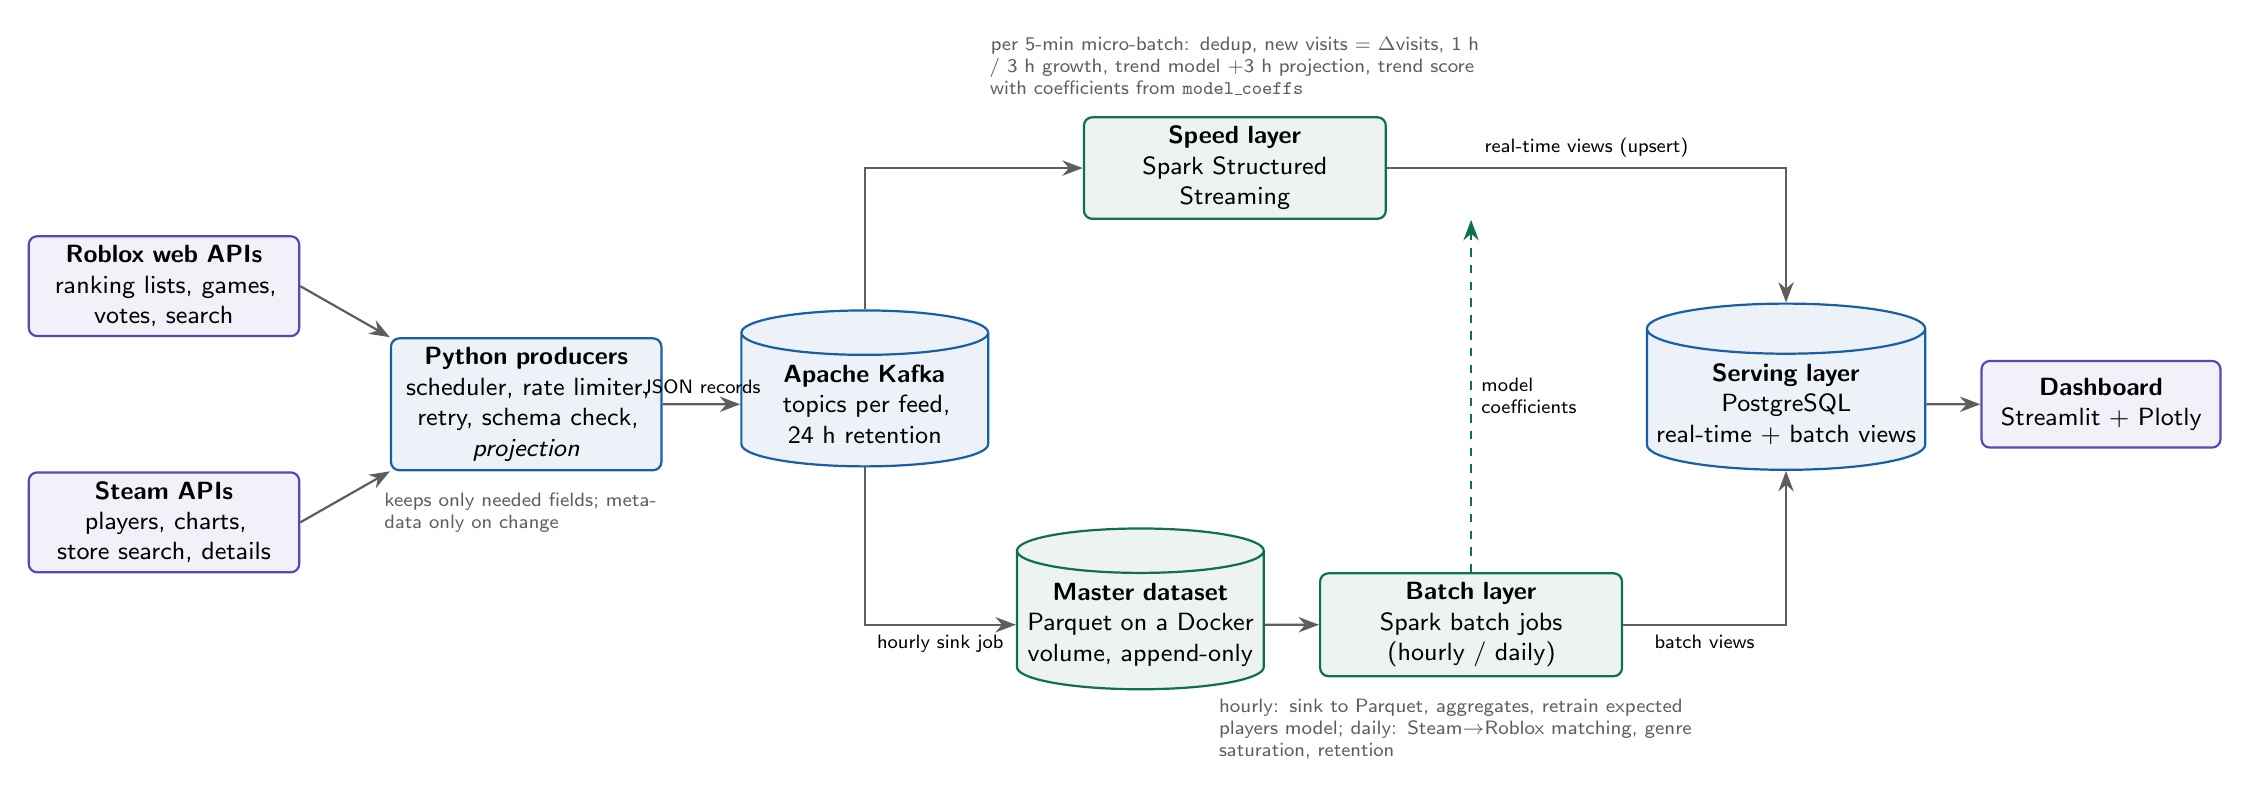
\begin{tikzpicture}[
  font=\sffamily\small,
  box/.style={rectangle, rounded corners=3pt, draw=#1, fill=#1!8, thick, align=center, minimum height=1.1cm, text width=3.2cm},
  box/.default=kfcgray,
  db/.style={cylinder, shape border rotate=90, aspect=0.18, draw=#1, fill=#1!8, thick, align=center, minimum height=1.3cm, text width=2.9cm},
  db/.default=kfcgray,
  arr/.style={-{Stealth[length=2.6mm]}, thick, draw=kfcgray},
  note/.style={font=\sffamily\scriptsize, align=left, text width=4.2cm, text=kfcgray}
]
% sources
\node[box=kfcpurple] (rb) at (0,2.1) {\textbf{Roblox web APIs}\\ranking lists, games,\\votes, search};
\node[box=kfcpurple] (st) at (0,-0.9) {\textbf{Steam APIs}\\players, charts,\\store search, details};
% ingestion
\node[box=kfcblue] (prod) at (4.6,0.6) {\textbf{Python producers}\\scheduler, rate limiter,\\retry, schema check,\\\emph{projection}};
\node[db=kfcblue] (kafka) at (8.9,0.6) {\textbf{Apache Kafka}\\topics per feed,\\24 h retention};
% speed layer
\node[box=kfcteal, text width=3.6cm] (speed) at (13.6,3.6) {\textbf{Speed layer}\\Spark Structured\\Streaming};
% batch layer
\node[db=kfcteal] (hdfs) at (12.4,-2.2) {\textbf{Master dataset}\\Parquet on a Docker\\volume, append-only};
\node[box=kfcteal, text width=3.6cm] (batch) at (16.6,-2.2) {\textbf{Batch layer}\\Spark batch jobs\\(hourly / daily)};
% serving
\node[db=kfcblue, text width=3.3cm] (pg) at (20.6,0.6) {\textbf{Serving layer}\\PostgreSQL\\real-time + batch views};
\node[box=kfcpurple, text width=2.8cm] (dash) at (24.6,0.6) {\textbf{Dashboard}\\Streamlit + Plotly};

\draw[arr] (rb.east) -- (prod.north west);
\draw[arr] (st.east) -- (prod.south west);
\draw[arr] (prod) -- node[above, font=\sffamily\scriptsize]{JSON records} (kafka);
\draw[arr] (kafka.north) |- (speed.west);
\draw[arr] (kafka.south) |- node[pos=0.75, below, font=\sffamily\scriptsize]{hourly sink job} (hdfs.west);
\draw[arr] (hdfs) -- (batch);
\draw[arr] (speed.east) -| node[pos=0.25, above, font=\sffamily\scriptsize]{real-time views (upsert)} (pg.north);
\draw[arr] (batch.east) -| node[pos=0.25, below, font=\sffamily\scriptsize]{batch views} (pg.south);
\draw[arr, dashed, draw=kfcteal] (batch.north) -- node[right, font=\sffamily\scriptsize, align=left]{model\\coefficients} (speed.south -| batch.north);
\draw[arr] (pg) -- (dash);

\node[note, above=0.15cm of speed, text width=6.2cm] {per 5-min micro-batch: dedup, new visits = $\Delta$visits, 1 h / 3 h growth, trend model +3 h projection, trend score with coefficients from \texttt{model\_coeffs}};
\node[note, below=0.15cm of batch, text width=6.4cm] {hourly: sink to Parquet, aggregates, retrain expected players model; daily: Steam$\to$Roblox matching, genre saturation, retention};
\node[note, below=0.15cm of prod, text width=3.6cm] {keeps only needed fields; metadata only on change};
\end{tikzpicture}
}
\caption{High-level data flow (lambda architecture).}
\label{fig:dfd}
\end{figure}

\textbf{Key assumptions.}
\begin{itemize}
  \item \textbf{Ingestion:} two producers (\ep{producer-roblox}, \ep{producer-steam}) with a scheduler, rate limiter, back-off on 429/5xx, schema check and field projection. Kafka topics: \ep{roblox.snapshots} (game stats and votes), \ep{roblox.sorts}, \ep{steam.players} and \ep{meta}, keyed by game ID, with 24\,h retention. The tracked set is games seen in ranking lists in the last 7 days plus clone candidates, capped at about 2,000 games.
  \item \textbf{Speed layer} (\ep{speed-job}: Spark Structured Streaming, local mode, 5-min trigger):
  \begin{itemize}
    \item deduplicate and validate records,
    \item compute new visits ($\Delta$visits) and 1\,h/3\,h growth,
    \item compute the trend model projection,
    \item compute the trend score with the latest coefficients from \ep{model\_coeffs},
    \item upsert the real-time views \ep{rt\_*}.
  \end{itemize}
  \item \textbf{Batch layer} (\ep{batch-sink} and \ep{batch-jobs}, scheduled inside the app image, no external orchestrator):
  \begin{itemize}
    \item \emph{hourly:} Kafka $\rightarrow$ append-only Parquet master dataset (Structured Streaming with \ep{availableNow} trigger and checkpoint, so nothing is lost or duplicated); aggregates and 24\,h/7\,d changes; retraining of the expected players model and saving of its coefficients to \ep{model\_coeffs},
    \item \emph{daily:} genre saturation, retention, and fully automatic Steam$\rightarrow$Roblox clone matching:
    \begin{itemize}
      \item candidates are Steam games released in the last 90 days with growing player counts; their titles are searched in the Roblox search API,
      \item hard rule: the Roblox game must be created after the Steam release,
      \item the match confidence (0--1) combines title similarity weighted by word rarity (TF--IDF over all Roblox titles, so generic words such as ``Legends'' count little) and the Steam title appearing in the Roblox description,
      \item only pairs above a confidence threshold are stored in \ep{bv\_*} and shown.
    \end{itemize}
    Matching precision is evaluated once by the team on a random sample of about 100 pairs.
  \end{itemize}
  \item \textbf{Serving layer:} PostgreSQL holds the real-time views \ep{rt\_*}, the batch views \ep{bv\_*}, \ep{model\_coeffs} and game metadata. The dashboard merges \ep{rt\_*} (recent hours) and \ep{bv\_*} (older data) in a single query.
\end{itemize}

\textbf{ML.} Both models use linear regression (Spark MLlib).
\begin{itemize}
  \item \textbf{Expected players model:} trained every hour on the last 7 days of hourly snapshots of all tracked games. It estimates how many players a game should have at a given time. The gap between actual and expected players is the \textbf{trend score}: games well above expectation are rising, and games well below are fading. It is evaluated with $R^2$ and RMSE.
  \item \textbf{Trend model:} fitted per game on its recent player counts in the speed layer. It gives the growth rate and a +3\,h projection. It is evaluated by MAE against two baselines, ``same as now'' and ``same time yesterday'', and the result is shown in the \emph{Model and data health} view.
\end{itemize}

\subsection{Data schema}

\textbf{Kafka topics.} Each record contains only the numeric fields needed for the speed layer; string metadata is published to \ep{meta} only on change. All topics use the game/app id as the message key.

{\small
\begin{longtable}{L{3.4cm} L{4.0cm} L{6.2cm}}
\toprule
\textbf{Topic} & \textbf{Key fields} & \textbf{Example values}\\
\midrule\endhead
\ep{roblox.snapshots} & \ep{ts, id, playing, visits,}\newline\ep{favorites, up, down} & \ep{ts}=1729208700, \ep{id}=7436755782, \ep{playing}=21\,496\\
\ep{roblox.sorts} & \ep{ts, country, rank, id,}\newline\ep{playerCount, isSponsored} & \ep{country}=``pl'', \ep{rank}=1\\
\ep{steam.players} & \ep{ts, appid, player\_count} & \ep{appid}=730, \ep{player\_count}=812\,345\\
\ep{meta} & \ep{ts, type, id, name,}\newline\ep{genre\_l1, created} & \ep{type}=``roblox'', \ep{name}=``Grow a Garden''\\
\bottomrule
\end{longtable}}

\textbf{PostgreSQL serving tables.}

{\small
\begin{longtable}{L{3.4cm} L{5.5cm} L{4.7cm}}
\toprule
\textbf{Table} & \textbf{Columns} & \textbf{Written by}\\
\midrule\endhead
\ep{rt\_game\_stats} & \ep{id, ts, playing, visits\_delta,}\newline\ep{growth\_1h, growth\_3h,}\newline\ep{trend\_score, projection\_3h} & speed layer (upsert, 5\,min)\\
\ep{rt\_ranked} & \ep{id, rank, platform, genre,}\newline\ep{country, ts} & speed layer (upsert, 5\,min)\\
\ep{bv\_history} & \ep{id, hour\_ts, avg\_playing,}\newline\ep{visits\_delta\_1h} & batch layer (hourly)\\
\ep{bv\_clones} & \ep{steam\_appid, roblox\_id,}\newline\ep{confidence, matched\_at} & batch layer (daily)\\
\ep{bv\_saturation} & \ep{genre\_l1, game\_count,}\newline\ep{total\_players, ts\_day} & batch layer (daily)\\
\ep{game\_meta} & \ep{id, platform, name, genre\_l1,}\newline\ep{genre\_l2, created, updated\_at} & producers (on change)\\
\ep{model\_coeffs} & \ep{trained\_at, intercept,}\newline\ep{coef\_json} & batch layer (hourly retrain)\\
\bottomrule
\end{longtable}}

%======================================================================
\section{Dashboard}
Streamlit + Plotly. It shows only what the sources provide. Growth, sparklines, projections and scores appear once enough history has been collected (hours to days).
\begin{figure}[H]
\centering
\resizebox{\textwidth}{!}{%
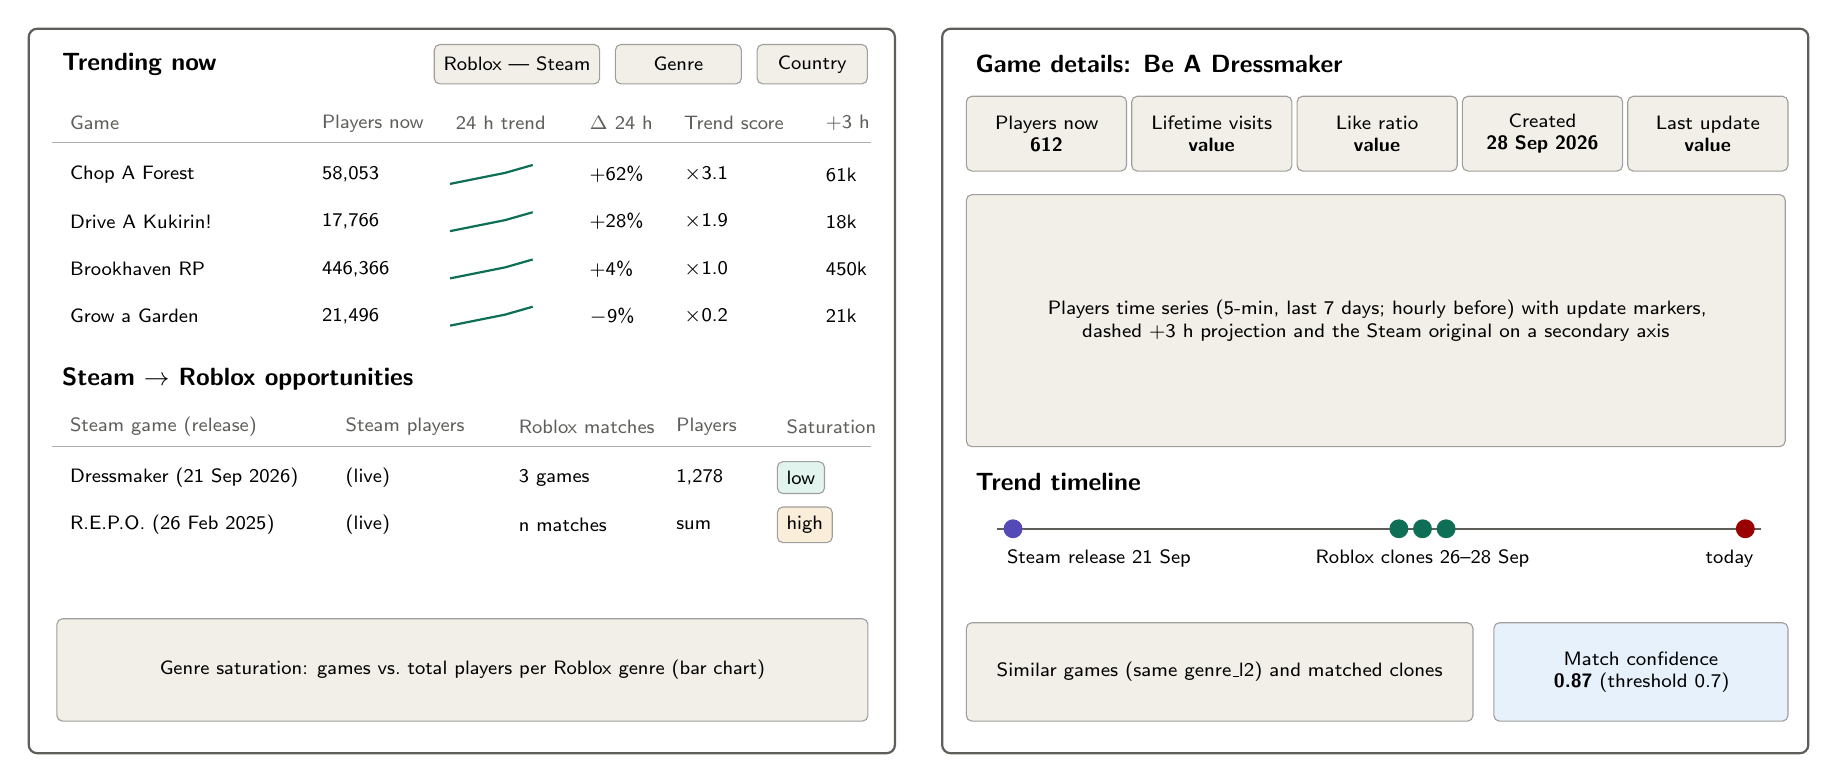
\begin{tikzpicture}[font=\sffamily\scriptsize,
  frame/.style={draw=kfcgray, thick, rounded corners=3pt},
  ph/.style={draw=kfcgray!60, fill=lightgray, rounded corners=2pt, align=center},
  hd/.style={font=\sffamily\bfseries\small}]
% ---- view 1
\draw[frame] (0,0) rectangle (11,9.2);
\node[hd, anchor=west] at (0.3,8.75) {Trending now};
\node[ph, minimum width=1.9cm, minimum height=0.5cm] at (6.2,8.75) {Roblox | Steam};
\node[ph, minimum width=1.6cm, minimum height=0.5cm] at (8.25,8.75) {Genre};
\node[ph, minimum width=1.4cm, minimum height=0.5cm] at (9.95,8.75) {Country};
\foreach \xx/\tx in {0.4/Game, 3.6/Players now, 5.3/24 h trend, 7.0/$\Delta$ 24 h, 8.2/Trend score, 10.0/+3 h} {\node[anchor=west, text=kfcgray] at (\xx,8.0) {\tx};}
\draw[kfcgray!50] (0.3,7.75) -- (10.7,7.75);
\foreach \yy/\nm/\pc/\dl/\sc/\pr in {7.35/Chop A Forest/58{,}053/+62\%/$\times$3.1/61k, 6.75/Drive A Kukirin!/17{,}766/+28\%/$\times$1.9/18k, 6.15/Brookhaven RP/446{,}366/+4\%/$\times$1.0/450k, 5.55/Grow a Garden/21{,}496/$-$9\%/$\times$0.2/21k} {
  \node[anchor=west] at (0.4,\yy) {\nm}; \node[anchor=west] at (3.6,\yy) {\pc};
  \draw[kfcteal, thick] (5.35,\yy-0.12) -- (5.7,\yy-0.05) -- (6.05,\yy+0.02) -- (6.4,\yy+0.12);
  \node[anchor=west] at (7.0,\yy) {\dl}; \node[anchor=west] at (8.2,\yy) {\sc}; \node[anchor=west] at (10.0,\yy) {\pr};}
\node[hd, anchor=west] at (0.3,4.75) {Steam $\rightarrow$ Roblox opportunities};
\foreach \xx/\tx in {0.4/Steam game (release), 3.9/Steam players, 6.1/Roblox matches, 8.1/Players, 9.5/Saturation} {\node[anchor=west, text=kfcgray] at (\xx,4.15) {\tx};}
\draw[kfcgray!50] (0.3,3.9) -- (10.7,3.9);
\node[anchor=west] at (0.4,3.5) {Dressmaker (21 Sep 2026)}; \node[anchor=west] at (3.9,3.5) {(live)}; \node[anchor=west] at (6.1,3.5) {3 games}; \node[anchor=west] at (8.1,3.5) {1,278}; \node[ph, fill=lightteal, anchor=west] at (9.5,3.5) {low};
\node[anchor=west] at (0.4,2.9) {R.E.P.O. (26 Feb 2025)}; \node[anchor=west] at (3.9,2.9) {(live)}; \node[anchor=west] at (6.1,2.9) {n matches}; \node[anchor=west] at (8.1,2.9) {sum}; \node[ph, fill=lightamber, anchor=west] at (9.5,2.9) {high};
\node[ph, minimum width=10.3cm, minimum height=1.3cm, anchor=south west] at (0.35,0.4) {Genre saturation: games vs.\ total players per Roblox genre (bar chart)};
% ---- view 2
\draw[frame] (11.6,0) rectangle (22.6,9.2);
\node[hd, anchor=west] at (11.9,8.75) {Game details: Be A Dressmaker};
\foreach \ii/\lb/\vl in {0/Players now/612, 1/Lifetime visits/value, 2/Like ratio/value, 3/Created/28 Sep 2026, 4/Last update/value} {
  \node[ph, minimum width=1.95cm, minimum height=0.95cm, anchor=north west, text width=1.8cm] at (11.9+\ii*2.1,8.35) {\lb\\\textbf{\vl}};}
\node[ph, minimum width=10.4cm, minimum height=3.2cm, anchor=north west, text width=10cm] at (11.9,7.1) {Players time series (5-min, last 7 days; hourly before) with update markers,\\dashed +3 h projection and the Steam original on a secondary axis};
\node[hd, anchor=west] at (11.9,3.45) {Trend timeline};
\draw[thick, kfcgray] (12.3,2.85) -- (22.0,2.85);
\fill[kfcpurple] (12.5,2.85) circle (0.12); \node[anchor=north west] at (12.3,2.7) {Steam release 21 Sep};
\fill[kfcteal] (17.4,2.85) circle (0.12); \fill[kfcteal] (17.7,2.85) circle (0.12); \fill[kfcteal] (18.0,2.85) circle (0.12);
\node[anchor=north] at (17.7,2.7) {Roblox clones 26--28 Sep};
\fill[red!60!black] (21.8,2.85) circle (0.12); \node[anchor=north] at (21.6,2.7) {today};
\node[ph, minimum width=6.4cm, minimum height=1.25cm, anchor=south west, text width=6.2cm] at (11.9,0.4) {Similar games (same genre\_l2) and matched clones};
\node[ph, fill=lightblue, minimum width=3.7cm, minimum height=1.25cm, anchor=south west, text width=3.5cm] at (18.6,0.4) {Match confidence\\\textbf{0.87} (threshold 0.7)};
\end{tikzpicture}
}
\caption{Wireframe of \emph{Trending now} and \emph{Game details}. Player counts and dates are real measurements from 17 Oct 2026. Growth, score, projection, saturation and match-confidence values are illustrative.}
\label{fig:wire}
\end{figure}

%======================================================================
\section{Infrastructure and technologies}
Everything runs locally with Docker Compose and needs about 8\,GB of RAM. There are two ready-made images (Kafka, PostgreSQL) and one own image, \ep{app}, which contains Python 3.12, Java 17 and Spark 3.5 with the Kafka connector and the PostgreSQL JDBC driver built in. The \ep{app} image is started as six services that differ only in their \ep{command}. This gives separate logs and restarts while there is still a single Dockerfile.
\begin{table}[H]
\centering\small
\begin{tabularx}{\textwidth}{L{3.0cm} L{3.4cm} Y}
\toprule
\textbf{Service} & \textbf{Image} & \textbf{Role}\\
\midrule
\ep{kafka} & \ep{apache/kafka:3.7.0} (KRaft) & message broker, 24\,h retention (1\,GB RAM)\\
\ep{postgres} & \ep{postgres:16} & serving layer: \ep{rt\_*}, \ep{bv\_*}, \ep{model\_coeffs}, metadata (512\,MB)\\
\ep{producer-roblox} & \ep{app} & ranking lists, games, votes every 5/15 min; search daily\\
\ep{producer-steam} & \ep{app} & current players every 15 min; charts, store search, details daily\\
\ep{speed-job} & \ep{app} & speed layer (Structured Streaming, \ep{spark.driver.memory} 2\,GB)\\
\ep{batch-sink} & \ep{app} & hourly Kafka $\rightarrow$ Parquet master dataset on volume \ep{/data/master}\\
\ep{batch-jobs} & \ep{app} & scheduled Spark batch jobs: aggregates, model training, matching (2\,GB)\\
\ep{dashboard} & \ep{app} & Streamlit on port 8501\\
\bottomrule
\end{tabularx}
\end{table}

\begin{table}[H]
\centering\small
\begin{tabularx}{\textwidth}{L{2.8cm} Y L{4.4cm}}
\toprule
\textbf{Layer} & \textbf{Chosen technology} & \textbf{Also considered}\\
\midrule
Ingestion & Python producers (\ep{requests}, \ep{confluent-kafka}, APScheduler) & Apache NiFi, Kafka Connect\\
Messaging & Apache Kafka 3.7 (KRaft, single broker) & Redpanda, RabbitMQ\\
Batch storage & Parquet + Snappy on a Docker volume & HDFS, MinIO (S3); switching only changes the storage path\\
Batch processing / ML & Apache Spark 3.5 (PySpark, local mode), Spark MLlib & Hive, Pandas\\
Stream processing & Spark Structured Streaming & Apache Flink, Kafka Streams\\
Scheduling & APScheduler inside the \ep{app} services & Apache Airflow, cron\\
Serving & PostgreSQL 16 & TimescaleDB, Cassandra\\
Presentation & Streamlit + Plotly & Grafana, Apache Superset\\
\bottomrule
\end{tabularx}
\end{table}

%======================================================================
\section{Risks and mitigations}

{\small
\begin{tabularx}{\textwidth}{L{4.2cm} L{2.0cm} Y}
\toprule
\textbf{Risk} & \textbf{Likelihood} & \textbf{Mitigation}\\
\midrule
Undocumented Roblox endpoints (\ep{explore-api}, \ep{search-api}) change or break & Medium & Fallback to documented legacy \ep{games.roblox.com} for player counts; alert on HTTP\,4xx; UUID \ep{sessionId} is stateless and trivially regenerated.\\
HTTP\,429 from Roblox (observed after ${\sim}$11 rapid requests) & High -- known & Per-endpoint back-off with jitter; batching up to 50 IDs per call; 1\,s sleep between batch groups.\\
Steam / SteamSpy throttling & Low & 0.5\,s sleep between per-game calls; store and \ep{appdetails} polled at daily cadence only.\\
Spark local-mode OOM on large micro-batches & Medium & \ep{spark.driver.memory 2g}; 5-min trigger limits in-flight data; \ep{maxOffsetsPerTrigger} for backpressure.\\
Clone matching false positives above threshold & Medium & Manual spot-check on ${\sim}$100 randomly sampled pairs before final demo; confidence threshold tunable in \ep{model\_coeffs}.\\
\bottomrule
\end{tabularx}}

%======================================================================
\section{Planned use of GenAI tools}
We will use \textbf{Claude Code} (Anthropic). The repository will contain:
\begin{itemize}
  \item a shared \ep{CLAUDE.md} with the architecture, Kafka topics, table schemas and coding conventions,
  \item a \emph{grill me} skill that critically questions each design or plan before implementation starts,
  \item dedicated implementation skills for recurring parts of the system, e.g.\ an API producer, a Spark Structured Streaming job, a Spark batch job, a new \ep{app} service in Docker Compose, and a Streamlit dashboard view.
\end{itemize}

%======================================================================
\noindent\begin{minipage}{\textwidth}
\section{Team and task allocation}
Each area has one owner (\textbf{O}) and two supporters (S).\par\vspace{6pt}
{\centering\small
\newcommand{\own}{\cellcolor{lightblue}\textbf{O}}
\begin{tabularx}{\textwidth}{Y >{\centering\arraybackslash}p{2.1cm} >{\centering\arraybackslash}p{2.1cm} >{\centering\arraybackslash}p{2.1cm} >{\centering\arraybackslash}p{2.1cm}}
\toprule
\textbf{Area} & \textbf{Bart\l{}omiej Borycki} & \textbf{Micha\l{} Iwaniuk} & \textbf{Jan Cwalina} & \textbf{Mi\l{}osz Choda\'n}\\
\midrule
Ingestion (Python producers) & & \own & S & S\\
Messaging (Kafka) & S & \own & & S\\
Batch storage (Parquet master dataset) & \own & S & S & \\
Batch processing / ML (Spark, MLlib) & S & & \own & S\\
Stream processing (Structured Streaming) & & S & S & \own\\
Scheduling and app image (APScheduler, Dockerfile, Compose) & S & S & \own & \\
Serving (PostgreSQL) & \own & & S & S\\
Presentation (Streamlit + Plotly) & S & S & & \own\\
\bottomrule
\end{tabularx}\par}
\end{minipage}

\end{document}
